\chapter{Banco de pruebas}\label{cap:bancopruebas}

	En este capítulo se describe el banco de pruebas en el que se va a verificar el funcionamiento del actuador. También se detallan algunas características del banco que son importantes para la etapa de diseño.

	El banco de pruebas elegido es la sala B039 del Departamento de Ingeniería Electrónica. En esta sala se guardan gran parte de los servidores que almacenan la informaci'on del departamento, por lo que se trata de un entorno real y adecuado para probar el actuador. Además, se encuentra monitorizado y está implementado una parte del sistema de monitorización explicado en el apartado \ref{sec:enfoque}. En la figura \ref{fig3_1:sala} se muestra una imagen de dicha sala.

En esta sala existen 2 sistemas de refrigeraci'on. Sus características son las siguientes:

\begin{itemize}
	\item\textbf{Sistema de refrigeraci'on del edificio:} su principal objetivo es mantener una temperatura de confort en cada una de las salas del edificio. Sin embargo, este sistema no es suficiente para evacuar el calor generado por los equipos, debido a que s'olo funciona durante los meses de verano. Además, no existe ningún mecanismo que permita controlar el sistema para que se pueda fijar la temperatura de esta sala según sus necesidades y de manera independiente al resto de salas del edificio. Por tanto, este sistema es descartado para el control de la temperatura.

	\item\textbf{Unidad de refrigeraci'on comercial:} su objetivo es la evacuaci'on del calor generado por los equipos de la sala. Este sistema funciona durante todo el a'no y permite configurar el \textit{setpoint}. Por tanto, el control de la temperatura se va a realizar utilizando este sistema.
\end{itemize}

\begin{figure}[h]
\centering
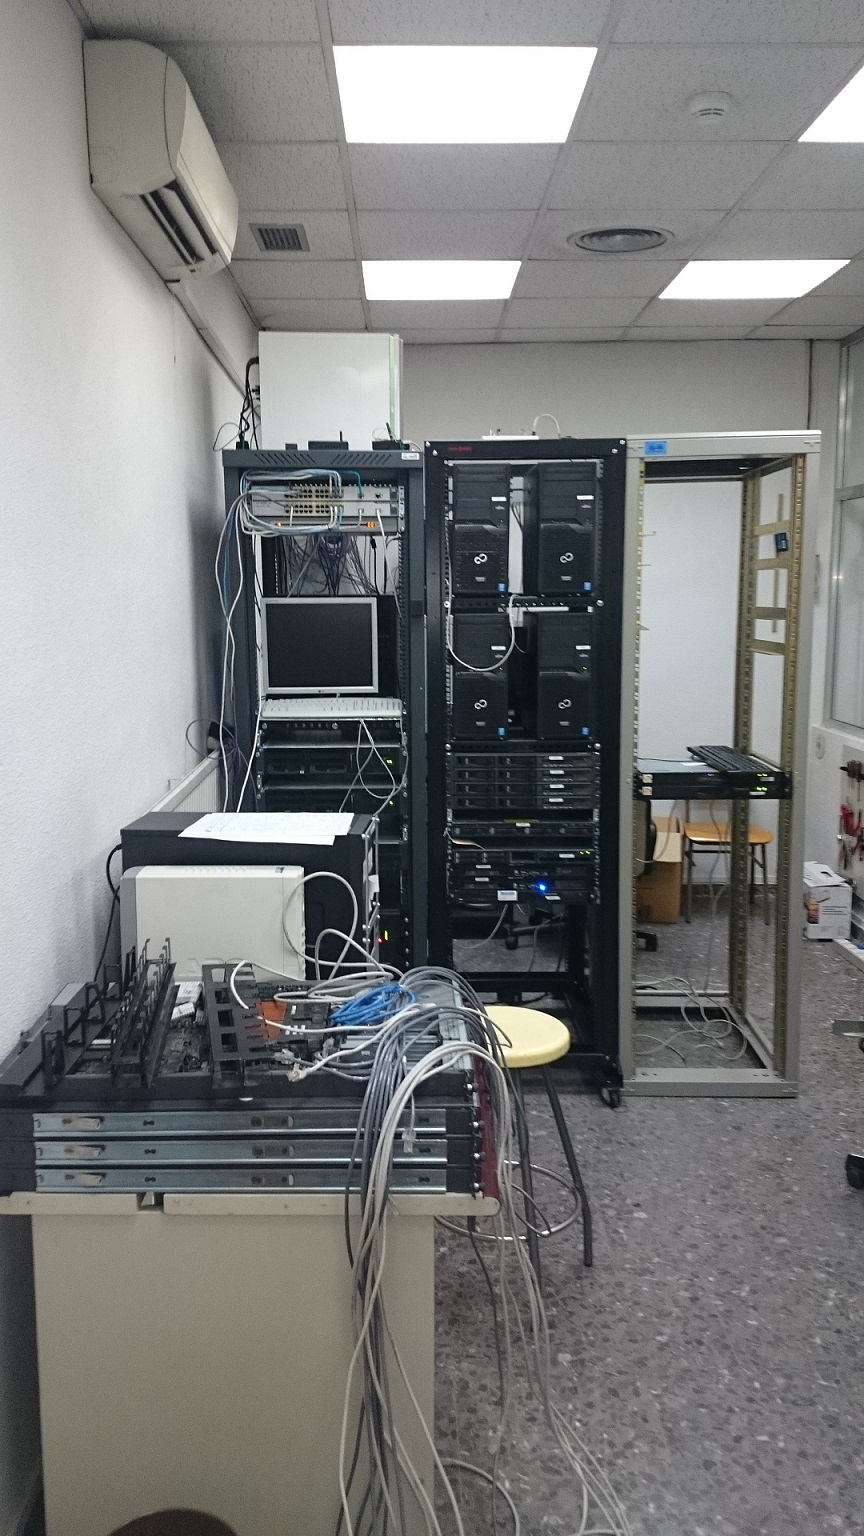
\includegraphics[width=0.55\textwidth,height=105mm]{imagenes/capitulo3/bancoPruebas2}
\caption {Fotograf'ia de la sala B039}
\label{fig3_1:sala}
\end{figure}

	El control del \textit{setpoint} se realiza de forma manual y a través de un mando a distancia. Este mando dispone de varias teclas que permiten configurar el modo de funcionamiento. Al pulsar alguna de estas teclas se envía una orden al sistema de refrigeración para que modifique su estado de funcionamiento.

	Cada una de las órdenes o modos de funcionamiento es representada a través de un comando. El comando está formado por una secuencia de bits con un determinado protocolo o formato que es interpretado por el receptor situado en la unidad de refrigeración. El receptor decodifica la secuencia recibida y en base a ello, modifica el funcionamiento del sistema de refrigeración.

	Cada comando es enviado al receptor mediante una señal de infrarrojos. Dicha señal está modulada a una frecuencia de 38 KHz, que es la frecuencia de portadora fijada por el fabricante para la comunicación a través del mando a distancia. El sistema posee un rango de funcionamiento que va de 18{$^\circ$}C a 32{$^\circ$}C, con saltos de 1{$^\circ$}C entre 2 temperaturas consecutivas. 

	Por tanto, la comunicación del sistema de actuación con la unidad de refrigeración deberá realizarse mediante un sistema de infrarrojos que emule el comportamiento del mando a distancia y que lo haga de manera automática. Además, deberá tener en cuenta las cuestiones mencionadas sobre el rango de funcionamiento y la modulación.






